\addtocounter{section}{1}
\section{Annex A: scripts and code}

This annex documents briefly the roles of each scripts and code files.

\subsection{Data generation}

See Table \ref{tab:annex-files-datagen}.

\begin{table}[h]
    \centering
    \begin{tabular}{|p{0.23\textwidth}|p{0.73\textwidth}|}
        \hline
        File name & Description \\ \hline
        \texttt{config.py} & Holds high level specification of the dataset to be created, such as the number of samples, the LHS strategy, and output files names. \\
        \texttt{read\_results.py} & Fetches the results from simulation directories, either one by one or all at once. \\
        \texttt{reference.py} & Runs the reference simulation and serializes the results in a json file. \\
        \texttt{sampling.py} & \texttt{--sample-only}: only run the LHS and store the samples in a CSV file. \texttt{--prepare-one idx}: prepares the simulation directory for one sample given its index. With no arguments, runs LHS and prepare all the simulation directories. \\
        \texttt{utils\_francois.py} & Stores the modified version of the \texttt{adjust\_capacity} function of Dispa-SET. \\ \hline
        \texttt{main.sh} & Starts all the scripts in the right order in order to produce a dataset. Runs the reference simulation, the sampling, prepends the header to the dataset file (as CSV), and starts the first series. \\
        \texttt{launch-job-series} \texttt{.sh} & Submits a series of simulation jobs, and a job that will submit the following series with the current one as a dependency. If the series index given as argument is too high, exits. \\
        \texttt{launch-reference-} \texttt{job.sh} & Submits a job that runs the reference simulation. \\
        \texttt{launch-simulation-} \texttt{jobs.sh} & Submits the jobs required to run a simulation from a series. It takes the series index as an argument and the number in that series from SLURM environment variables. Uses \texttt{sampling.py --prepare-one}, GAMS and \texttt{read\_results.py} successively. \\
        \texttt{gams-simulation.sh} & Submits a job running the GAMS simulation of an already prepared simulation, for testing purposes. \\
        \texttt{read-one.sh} & Submits a job fetcing the results of an arleady ran GAMS simulation, for testing purposes. \\
        \texttt{get-longest-} \texttt{simulation.sh} & Bash script that calls the \texttt{seff} utility on each of the simulation ran to extract the longest ones. This has mainly be used once to set the simulation timeout that prevent stalling simulation to waste resources. \\ \hline
    \end{tabular}
    \caption{Description of the data-generation files}
    \label{tab:annex-files-datagen}
\end{table}

\subsection{Neural network}

See Table \ref{tab:annex-files-nn}.

\begin{table}[h]
    \centering
    \begin{tabular}{|p{0.21\textwidth}|p{0.75\textwidth}|}
        \hline
        File name & Description \\ \hline
        \texttt{config.py} & Holds the configuration of the network to be trained, name, data to use, inputs and outputs. \\
        \texttt{model.py} & Holds the description of the model to be trained, via the \texttt{build\_model} function. \\
        \texttt{baselines.py} & Builds and trains different, predefined neural network architectures, and stores their performance. This eases the process of looking for a good architecture for the ANN, to guide the bounds in the hyper-parameter tuning. With \texttt{sort -k2 -t '>' -i logs\/baselines-results.txt} one easily sorts the results by increasing order. \\
        \texttt{train.py} & Executes the tuner search for the best model and training of that best model. \\
        \texttt{view.py} & Holds different utilities to view the results of some model and its performance. Use \texttt{view.py --surface <in1> <in2> <out>} to create a 3D surface of the out-th output depending on the in1 and in2-th inputs. The other inputs are constant and parameterizable with sliders. \\
        \hline
    \end{tabular}
    \caption{Description of the files for the neural network part.}
    \label{tab:annex-files-nn}
\end{table}

\subsection{Integration}

See Table \ref{tab:annex-files-integration}.

\begin{table}[h]
    \centering
    \begin{tabular}{|p{0.21\textwidth}|p{0.75\textwidth}|}
        \hline
        File name & Description \\ \hline
        \texttt{external.h} & Header file for \texttt{external.cpp}. \\
        \texttt{external.cpp} & Main source file for the library. \\
        \texttt{main.cpp} & Code for running a test program. \\
        \texttt{Makefile} & GNU make file for automating compilation. \\
        \texttt{tensorflow.dll} & Tensorflow library file for Windows, can be downloaded from \href{https://www.tensorflow.org/install/lang_c}{here}. \\
        \hline
    \end{tabular}
    \caption{Description of the integration files.}
    \label{tab:annex-files-integration}
\end{table}

\newpage
\section{Annex B: Dispa-SET components and representation}

Dispa-SET provides us with several predefined configurations, each of these defining the zones and their units of interest, and linking to the relevant data (e.g. times series provided as \texttt{csv} files).

In this work, the european setting is used, that is, the zones simulated correspond approximately to the European Union.

\subsection{Zones}

Most of the EU contries are represented, for completeness they are reported in Table \ref{table:countries-eu}.

\begin{table}[h]
    \centering
	\begin{tabular}{|l l|l l|}
		\hline
		Code & Country & Code & Country \\
		\hline
		AT & Austria        & IE & Ireland \\
		BE & Belgium        & IT & Italy \\
		BG & Bulgaria       & LT & Lithuania \\
		CH & Switzerland    & LV & Latvia \\
		CZ & Czech Republic & NL & Netherlands \\
		DE & Germany        & NO & Norway \\
		DK & Denmark        & PL & Poland \\
		EE & Estonia        & PT & Portugal \\
		EL & Greece         & RO & Romania \\
		ES & Spain          & SE & Sweden \\
		FI & Finland        & SI & Slovenia \\
		FR & France         & SK & Slovakia \\
		HR & Croatia        & UK & United Kingdom \\
		HU & Hungary        & & \\
		\hline
	\end{tabular}
	\caption{Countries present in Dispa-SET EU, and their ISO Alpha 2 country codes. These are all the EU contry except for Cyprus and Malta and Luxembourg, plus Norway, Switzerland and the UK.}
	\label{table:countries-eu}
\end{table}

\subsection{Technologies}

Table \ref{table:technologies-eu} lists all the technologies taken into account by Dispa-SET, alongside with their main properties: 

\begin{itemize}
    \item VRES: does the technology belongs to VRES?
    \item Storage: can it store energy?
    \item Flexibility: ease of control of the unit's power output.
\end{itemize}

Due to the intermittency of their resources, and because one cannot dispatch them, VRES are considered inflexible.

However, hydroelectric units with a reservoir are have some room for flexibility, due their ability to manage their storage level.

Steam turbines, because of their dependency on the fuel used, e.g. nuclear energy would be less flexible than natural gas.

Heating and combined heat and power units are not covered, as only the electricity is of interest in this scope.

\begin{table}
    \centering
    \begin{tabular}{|l l c c c|}
        \hline
		Identifier & Description & VRES & Storage & Flexibility\\
		\hline
		COMC & Combined cycle             & No  & No  & High\\
		GTUR & Gas turbine                & No  & No  & High\\
		ICEN & Internal combustion engine & No  & No  & High\\
		STUR & Steam turbine              & No  & No  & Medium\\
		HDAM & Conventional hydro dam     & No  & Yes & Medium \\
		HROR & Hydro run-of-river         & Yes & No  & Low\\
		HPHS & Pumped hydro storage       & No  & Yes & Medium\\
		WTOF & Offshore wind turbine      & Yes & No  & Low\\
		WTON & Onshore wind turbine       & Yes & No  & Low\\
		PHOT & Solar photovoltaic         & Yes & No  & Low\\
		BATS & Stationary batteries       & No  & Yes & High\\
		\hline
    \end{tabular}
    \caption{Technologies present in Dispa-SET}
    \label{table:technologies-eu}
\end{table}


\subsection{Fuels}

Table \ref{table:fuels-eu} summarizes the fuel types in Dispa-SET.

It is important to highlight that technologies may not always be powered by the same fuel, for instance, the steam turbines can use most of them.

Each unit must specify its technology and fuel. Depending on the optimization problem formulation, units featuring the same (technology-fuel) pair will be grouped together and thereafter be treated as one single unit. This grouping is of crucial importance, as it will define the behaviour of the simulation when using the MILP formulation (see \ref{subsubection:milp}).

\begin{table}[h]
    \centering
	\begin{tabular}{|l l|}
		\hline
		Fuel & Description\\
		\hline
		BIO & Biofuels\\
		GAS & Gas\\
		HRD & Coal\\
		LIG & Lignite \\
		NUC & Nuclear energy\\
		OIL & Petroleum\\
		PEA & Peat Moss\\
		GEO & Geothermal steam \\
		SUN & Solar energy\\
		WAT & Hydro energy\\
		WIN & Wind energy\\
		WST & Energy from waste\\
		OTH & Other fuels and energy carriers\\
		\hline
	\end{tabular}
	\caption{Fuel types in Dispa-SET}
	\label{table:fuels-eu}
\end{table}

A major consideration for the optimization problem is the fuel prices, which are listed in Table \ref{table:fuel-prices}.

A key feature is the relationship between the price of coal and the price of gas: depending on which one is the cheaper, the optimal behaviour change dramatically. Obviously, the cheapest one will always be preferred over the other when choice arise. 

\begin{table}[h]
    \centering
	\begin{tabular}{|l c|}
		\hline
		& Price \\
		\hline
		Nuclear    & 3 \\
		Black coal & 20 \\
		Gas        & 45 \\
		Fuel-Oil   & 65\\
		Biomass    & 10.08\\
		Lignite    & 7.23\\
		Peat       & 9.36 \\
		\hline
	\end{tabular}
	\caption{Fuel prices considered, in €/MWh}
	\label{table:fuel-prices}
\end{table}

\subsection{Other prices}

Some other price values are relevant, such as the price of the load shedding per MWh. These are presented in Table \ref{table:other-prices}.

\begin{table}[h]
    \centering
	\begin{tabular}{|l c|}
		\hline
		What & Price \\
		\hline
		CO2                & 25 \\
		Unserved Heat      & 84.21\\
		Load Shedding Cost & 1000\\
		Transmission       & 0\\
		Unserved H2        & 75\\
		Curtailment Cost   & 20 \\
		\hline
	\end{tabular}
	\caption{Other relevant prices, in €/MWh}
	\label{table:other-prices}
\end{table}

\mywarning{prix du CO2 en euro/MWh}

These values define the significance of each problem relatively to each other, hence what option is the least costly. For instance, the shedding cost could be so low compared to the carbon emissions that it is preferable not to run any coal unit to produce 1MW than to shed 1MW. This example is extreme, but outlines the fact that these prices impact the simulation outcome via their use in the objective function.

\subsection{Power plants}

As a dispatch model, Dispa-SET evidently has to model the units it dispatches, namley the power plants that are present in each of the modelled zones.

For performance reasons, some of the units initially described are merged into clustered units at the pre-processing step. Thus, the amount of variable in the simulation is reduced, while the accuracy is not significantly impacted \cite{dispaset}.

Dispa-SET disposes of utilities to do so, but also needs to craft the new, aggregated units properties table. These are defined by the set of feilds that are shown in Table \ref{table:plant-db}.

\begin{table}[h]
    \centering
    \begin{tabular}{|l l l|}
        \hline
        Field           & Description                       & Type                    \\ \hline
        Unit            & Unit name                         & string                  \\
        PowerCapacity   & Maximum power output              & value in MW             \\
        Nunits          & Number of initial units clustered & integer                 \\
        Zones           & The unit's zone                   & string                  \\
        Fuel            & The fuel used                     & string                  \\
        Efficiency      & The unit's efficiency             & real in [0,1]           \\
        MinEfficiency   & Efficiency at minimum load        & real in [0,1]           \\
        MinUpTime       & Minimum up time                   & value in hours          \\
        MinDownTime     & Minimum down time                 & value in hours          \\
        RampUpRate      & Ramp up rate                      & value in minute$^{-1}$  \\
        RampDownRate    & Ramp down rate                    & value in minute$^{-1}$  \\
        RampingCost     & Cost of ramping up or down        & value in €/hour         \\
        StartUpCost\_pu & Start up cost per clustered unit  & value in €              \\
        NoLoadCost\_pu  & Cost of having no load on a unit  & value in €/hour         \\
        PartLoadMin     & Ratio of the minimum nominal capacity & real in [0,1]       \\
        StartUpTime     & Time to start up the plant        & value in hour           \\
        CO2Intensity    & Amount of CO$_2$ emitted per MW   & value in €/MW           \\ \hline
    \end{tabular}
    \caption{The table fields used to describe a optionnally aggregated power plant unit}
    \label{table:plant-db}
\end{table}

For the storage units, one needs some more parameters, given in Table \ref{table:plant-storage-db}. These feilds will remain blank for the other unit types.

\begin{table}[h]
    \centering
    \begin{tabular}{|l l l|}
        \hline
        Field                 & Description                       & Type          \\ \hline
        STOCapacity           & The total energy storage capacity & value in MWh  \\
        STOSelfDischarge      & The discharge rate (w.r.t. to the total) & value in day$^{-1}$ \\
        STOMaxChargingPower   & Maximum energy inflow             & value in MW   \\
        STOChargingEfficiency & The unit's charging efficiency    & real in [0,1] \\ \hline
    \end{tabular}
    \caption{Fields describing the storage capabilities of the units}
    \label{table:plant-storage-db}
\end{table}


Their discharge efficiency will be assigned to the common Efficiency field, and the PowerCapacity will be assigned the power output on discharge.

For batteries units, the RampUpRate and RampDownRate fields are set to 1, while the others but efficiency are set to 0. 

The crucial capability of storage units is their storage volume. In previous work in this context, the number of hours a unit can run at maximum output capacity is fixed as 4 hours, thus implicitly fixing a storage capacity given a power output.

This choice is arbitrary and leads to a simplification of the reality, where one could find huge differences in this ratio. To remove this, an option is added in Dispa-SET's adjusting function, to be able to filter the adjustments by range, making it now able to discriminate the units based on the storage capacity over maximum output power ratio, enabling its use to adjust storage units with different "longevity" separately.

However in reality, most of the difference is between the pumped hydro storage, that can typically output their maximum power for a longer time, and the other storage technologies, such as batteries.

At the end, this differenciation is not done, as it would also require the inputs of the surrogate model to be changed, to take into account the share of "high-longevity" storage units with respect to the "low-lengevity" ones.

\subsection{Notes on the other inputs}

We can make a few miscellaneous remarks about Dispa-SET input data.

\begin{itemize}
    \item The electricity demand is a time series from year 2019, per zone. It is assumed to be independent of the price.
    \item The net transfer capacities (NTC) between the different zones are given as inputs as hourly times series over a year. Then the maximum is picked and it is assumed that it remains constant over the year.
    \item The availability factors (AF) for renewable energy sources, defined as the ratio of the nominal power that is possible to output hourly. It is given as an hourly time series (adimentional).
    
    This variable energy generation is either curtailed or sent to the grid.

    Non-renewable technologies have their AF set to 1.

    In this work, AF denotes the hourly capacity factor, and CF (Capacity Factor) refers to the annual value. Hence, the capacity factor is the yearly average of the availability factor. 
\end{itemize}

\newpage
\section*{Appendix C: Vensim models}

Vensim offers a variety of tools to describe models, but at the end every model is an interconnection of variables, the math hiding in the connections between these. 

Vensim provides the following types of variables:
\begin{itemize}
    \item \textbf{Auxiliary variables}, that are regular variable that have no memory, that is, are independent from their value at the previous time step and are computed from every type of variable.

    For example, a $temperature$ variable that is computed from some $sunshine$ and $latitude$, that is used to compute the birth rate of $rabbits$ and $foxes$.

    \item \textbf{Constant variables}, that hold one value.
    
    For example, a mathematical constant like $\pi$.

    \item \textbf{Data variables}, or exogenous variables, whose value evolve over time but is not dependent of the model.

    For example, typical $sunshine$ data over a year.

    \item \textbf{Stock variables}, that change only over time as a function of the incoming rates, i.e., they integrates the rates.

    For example, the population of some species at a given time.

    \item \textbf{Rate variables}, or flows, that directly impact the Stock variables. 

    For example, the birth or death rate of some population at a given time.
\end{itemize}

The connections between the variables are virtually done by arrows. The only practical use of arrows is to make the variable at the origin appear in the selection of variables in the variable equation screen for the variable pointed by the arrow. But obviously they are of great utility in terms of visualization of the model.

An illustrative example of a Vensim model is depicted in Figure \ref{fig:vensim-model-example}.

\begin{figure}[h!]
    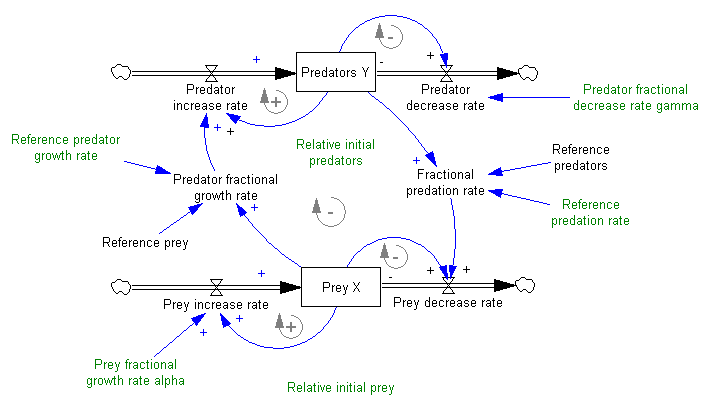
\includegraphics[width=0.9\textwidth]{resources/images/vensim-model-example.png}
    \caption{An example model in Vensim: Lotka-Volterra predator-prey model.}
    \label{fig:vensim-model-example}
\end{figure}